% !TeX root = ../main.tex

\chapter{数据分析}

\section{数据处理流程}

\subsection{数据解包、信息提取}
\label{sec:data_unpack}
DPU 通过 SiTCP 上传的数据文件格式为 \texttt{.dat},每个文件包含一次测量的所有数据帧。数据帧有两种类型,一种是波形信息,另一种是时间幅度提取信息,两种信息的数据帧格式如图 \ref{fig:data_format} 所示。
\begin{figure}[htbp]
    \centering
    \begin{subfigure}[t]{0.35\textwidth}
        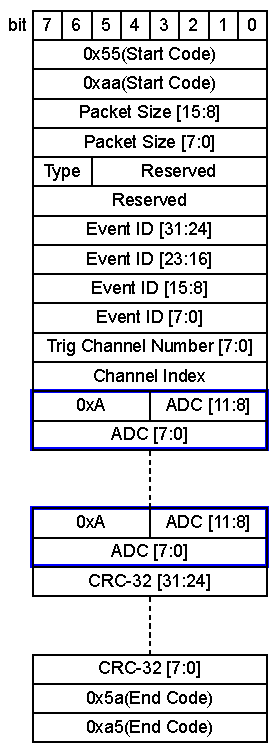
\includegraphics[width=\textwidth]{DPU_v0-DATA Format_WV.drawio.pdf}
        \caption{包含波形信息的数据帧(一个数据帧包括一个电子学通道的 1024 个波形数据点)}
        \label{fig:data_format_wv}
    \end{subfigure}
    \hfill
    \begin{subfigure}[t]{0.35\textwidth}
        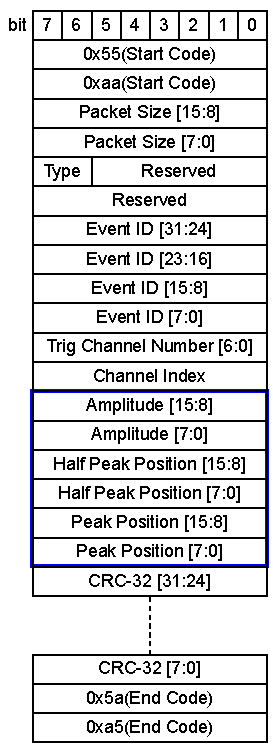
\includegraphics[width=\textwidth]{DPU_v0-DATA Format_TQ.drawio.pdf}
        \caption{包含时间幅度提取信息的数据帧(一个数据帧包括一个电子学通道波形的幅度、半峰值时间、峰值时间提取信息)}
        \label{fig:data_format_tq}
    \end{subfigure}
    \caption{数据帧格式}
    \label{fig:data_format}
\end{figure}

将上述感兴趣的数据统一存入名为 \verb|Packet| 的结构体中,其结构如下:
% \begin{minted}[linenos, breaklines, breakafter=/]{c++}
\begin{verbatim}
struct Packet
{
    uint8_t u8Type = 0;
    uint32_t u32EventID = 0;
    uint8_t u8TrigChaNum = 0;
    uint8_t u8ChannelIndex = 0;
    uint16_t au16ADC[Config::ADCPOINTS] = {};
    uint16_t u16Amplitude = 0;
    uint16_t u16HalfTime = 0;
    uint16_t u16PeakTime = 0;
};
\end{verbatim}
% \end{minted}

如果数据帧为波形信息,先判断波形数据是否饱和,如果饱和则将饱和部分的数据点进行拟合。其中波形前沿使用线性拟合,波形后沿使用指数拟合,拟合函数如下:
\begin{equation}
    f(x) = \left\{
    \begin{aligned}
        & a \cdot x + b, & x \leq x_0, \\
        & c \cdot \exp(-d \cdot x) + e, & x > x_0.
    \end{aligned}
    \right.
\end{equation}

然后,对波形数据进行信息提取,包括波形的幅度、半峰值时间、峰值时间等信息。最后,将波形提取信息或时间幅度提取信息存入名为 \verb|TreeEntry| 的结构体中,再将其以以下结构写入 ROOT 文件中。
% \begin{minted}[linenos, breaklines, breakafter=/]{C++}
\begin{verbatim}
tTree = new TTree("tTree", "Tree for data extraction");

tTree->Branch("EventID", &sTreeEntry.iEventID, Form("EventID/I"));
tTree->Branch("TriggerChannelNumber", &sTreeEntry.iTrigChaNum, Form("TriggerChannelNumber/I"));
tTree->Branch("ChannelIndex", sTreeEntry.aiChannelIndex, Form("ChannelIndex[%d]/I", Config::CHANNELNUM));
tTree->Branch("ADC", sTreeEntry.viADC.data());  // Do not store ADC data in the tree.
//tTree->Branch("ADC", &sTreeEntry.viADC);  // If ADC data is usefull, use this line.
tTree->Branch("EventIndex", &sTreeEntry.iEventIndex, Form("EventIndex/I"));
tTree->Branch("MeanOfBaseline", sTreeEntry.aiMeanOfBaseline, Form("MeanOfBaseline[%d]/I", Config::CHANNELNUM));
tTree->Branch("SubMeanOfBaseline", sTreeEntry.aiSubMeanOfBaseline, Form("SubMeanOfBaseline[%d]/I", Config::CHANNELNUM));
tTree->Branch("SigmaOfBaseline", sTreeEntry.aiSigmaOfBaseline, Form("SigmaOfBaseline[%d]/I", Config::CHANNELNUM));
tTree->Branch("Amplitude", sTreeEntry.aiAmplitude, Form("Amplitude[%d]/I", Config::CHANNELNUM));
tTree->Branch("HalfTime", sTreeEntry.aiHalfTime, Form("HalfTime[%d]/I", Config::CHANNELNUM));
tTree->Branch("PeakTime", sTreeEntry.aiPeakTime, Form("PeakTime[%d]/I", Config::CHANNELNUM));
tTree->Branch("Peak2Peak", sTreeEntry.aiPeak2Peak, Form("Peak2Peak[%d]/I", Config::CHANNELNUM));
tTree->Branch("SumOfAmplitude", &sTreeEntry.iSumOfAmplitude, Form("SumOfAmplitude/I"));
\end{verbatim}
% \end{minted}

\subsection{反符合剔除}
\label{sec:anti_coincidence}
将 \ref{sec:data_unpack} 节中保存的 ROOT 文件中的数据进行反符合剔除,剔除方法为:依次遍历每个事例,再对每个事例中的每个通道的通道号进行判断,如果通道号对应的 Map 为反符合通道,则将该事例整体剔除。剔除后的数据保存在新的 ROOT 文件中。

\subsection{特征提取}
\subsubsection{特征}
对 \ref{sec:anti_coincidence} 剔除后的数据或 \ref{sec:data_unpack} 的数据进行特征提取,提取的特征包括:
\begin{itemize}
    \item 事例总幅度
    \item X 维击中数
    \item Y 维击中数
    \item X\&Y 维击中数矢量和
    \item X\&Y 维击中数差
    \item 事例各通道最大峰值时间和最小峰值时间之差
    \item X 维最远击中位置
    \item Y 维最远击中位置
    \item 事例最大能量沉积的相对时间位置
    \item $\theta$ 入射角
    \item $\phi$ 入射角
    \item X 维 Pearson 相关系数
    \item Y 维 Pearson 相关系数
    \item X 维径迹长度
    \item Y 维径迹长度
    \item 单位距离能量沉积
    \item 是否击中边缘通道
\end{itemize}
%ROOT 文件结构如下:
%\begin{minted}[linenos, breaklines, breakafter=/]{C++}
%tFeaturesTree = new TTree("tFeaturesTree", "Features Tree");
%tFeaturesTree->Branch("EnergyOfEvent", &sFeatures.iEnergyOfEvent, "EnergyOfEvent/I");
%tFeaturesTree->Branch("XHitCount", &sFeatures.iXHitCount, "XHitCount/I");
%tFeaturesTree->Branch("YHitCount", &sFeatures.iYHitCount, "YHitCount/I");
%tFeaturesTree->Branch("SumHitCount", &sFeatures.fSumHitCount, "SumHitCount/F");
%tFeaturesTree->Branch("HitCountDiff", &sFeatures.iHitCountDiff, "HitCountDiff/I");
%tFeaturesTree->Branch("TimeDiff", &sFeatures.iTimeDiff, "TimeDiff/I");
%tFeaturesTree->Branch("XStartPos", &sFeatures.iXStartPos, "XStartPos/I");
%tFeaturesTree->Branch("YStartPos", &sFeatures.iYStartPos, "YStartPos/I");
%tFeaturesTree->Branch("BraggPeakPos", &sFeatures.fBraggPeakPos, "BraggPeakPos/F");
%tFeaturesTree->Branch("IncidentAngle", &sFeatures.fIncidentAngle, "IncidentAngle/F");
%tFeaturesTree->Branch("PhiAngle", &sFeatures.fPhiAngle, "PhiAngle/F");
%tFeaturesTree->Branch("XPearsonCorrCoef", &sFeatures.fXRho, "XRho/F");
%tFeaturesTree->Branch("YPearsonCorrCoef", &sFeatures.fYRho, "YRho/F");
%tFeaturesTree->Branch("XTrackLength", &sFeatures.fXTrackLength, "XTrackLength/F");
%tFeaturesTree->Branch("YTrackLength", &sFeatures.fYTrackLength, "YTrackLength/F");
%tFeaturesTree->Branch("dEdx", &sFeatures.fdEdx, "dEdx/F");
%tFeaturesTree->Branch("HitBoundary", &sFeatures.bHitBoundary, "HitBoundary/O");
%\end{minted}

\subsubsection{数据筛选}
对特征提取后的数据进行筛选,筛选条件为:X/Y 维击中数为 0、X\&Y 维径迹长度小于 2 (这里径迹长度的算法有问题,待修正)和击中位置在膜窗外的事例。筛选后的数据保存在新的 ROOT 文件中。

\subsection{TMVA 训练}
使用 BDT(Bosted Decision Tree) 方法进行训练,训练的特征包括:
\begin{itemize}
    \item 事例总幅度
    \item X 维击中数
    \item Y 维击中数
    %\item X\&Y 维击中数矢量和
    %\item X\&Y 维击中数差
    \item 事例各通道最大峰值时间和最小峰值时间之差
    \item X 维最远击中位置
    \item Y 维最远击中位置
    \item 事例最大能量沉积的相对时间位置
    \item $\theta$ 入射角
    %\item $\phi$ 入射角
    \item X 维 Pearson 相关系数
    \item Y 维 Pearson 相关系数
    \item X 维径迹长度
    \item Y 维径迹长度
    \item 单位距离能量沉积
    %\item 是否击中边缘通道
\end{itemize}

\subsection{TMVA 测试}
用 TMVA 训练好的 BDT 方法对测试数据进行测试,测试数据的特征提取方法与训练数据相同。测试结果保存在 ROOT 文件中。

\section{数据分析结果}

\subsection{使用前期阳极条两两合并的数据进行训练}
\begin{table}[!htbp]
    \centering
    \caption{阳极条两两合并的数据训练结果}
    \label{tab:big}
    \begin{tabular}{c c c}
    \toprule
    源类型                  &   $\mathrm{^{90}Sr}$      &   本底    \\
    \midrule
    工作气体                &   $\mathrm{C_4H_{10}}$    &   $\mathrm{C_4H_{10}}$    \\
    高压 [V]                &    370                    &   370 \\
    时间戳                  &   20240804231807          &   20240807112240  \\
    测试时间                &   2min                    &   9h  \\
    原始计数                &   150293                  &   299061  \\
    去除反符合计数          &   147597                  &   227822  \\
    去除单维事例计数        &   147597                  &   227812  \\
    去除短径迹、膜窗外计数  &   142647                  &   41313   \\
    BDT 筛选后计数(率)    &   85637(714 cps)          &   4339(8.0 cpm)\\
    发射率 [$s^{-1}$]       &   --                      &   --  \\
    保留/剔除率 [\%]               &   57                      &   98.5  \\
    阈值                    &   0.06                    &   0.06    \\
    类型                    &   WV 训练数据             &   WV 训练数据 \\
    \bottomrule
    \end{tabular}
\end{table}

\subsection{使用太原标准源中心阳极条测试数据进行训练(见表 \ref{tab:bigCentreSr90}、\ref{tab:bigCentreCl36} 和 \ref{tab:bigCentreAm241})}
\begin{table}[!htbp]
    \centering
    \caption{太原标准 $\mathrm{^{90}Sr}$ 源中心阳极条测试数据训练结果}
    \label{tab:bigCentreSr90}
\resizebox{\textwidth}{!}{
    \begin{tabular}{c c c c c}
    \toprule
    源类型                  &   $\mathrm{^{90}Sr}$      &   本底    &   $\mathrm{^{90}Sr}$  &   本底    \\
    \midrule
    工作气体                &   $\mathrm{CO_2}$    &   $\mathrm{CO_2}$    & $\mathrm{CO_2}$ &   $\mathrm{CO_2}$\\
    高压 [V]                &    540                    &   540 &   540 &   540 \\
    时间戳                  &    \makecell[c]{20240906172844 \\ 20240906180546 \\ 20240906180839 \\ 20240906181151 \\ 20240906181440}         &   \makecell[c]{20240923194604 \\ 20240924214355}  & \makecell[c]{20240906181811 \\ 20240906185136 \\ 20240906185441 \\ 20240906185732 \\ 20240906190011}    &   20240925200257  \\
    测试时间                &   \SI{10}{min}                    &   \SI{24}{h}  &   \SI{10}{min}    &   \SI{12}{h}  \\
    原始计数                &   592221                  &   449884  &   591632  &   225801  \\
    去除反符合计数          &   587572                  &   412595  &   586741  &   207047  \\
    去除单维事例计数        &   586408                  &   321045  &   585652  &   160728  \\
    \makecell[c]{去除短径迹、\\膜窗外计数}  &   568140                  &   146392   &  567579  &   74081   \\
    BDT 筛选后计数(率)    &   397135(\SI{661.9}{cps})          &   1544(\SI{1.1}{cpm})    &   398677(\SI{664.5}{cps}) &   888(\SI{1.2}{cpm})  \\
    发射率 [$s^{-1}$]       &   1190                      &   --  & 1190    &   --  \\
    效率 [\%]               &   55.6                      &   99.6  &   55.8    &   99.6    \\
    阈值                    &   0.12                    &   0.12    &   0.12    &   0.12    \\
    类型                    &   TQ 训练数据             &   WV 训练数据 &   TQ 测试数据 &   WV 测试数据 \\
    \bottomrule
    \end{tabular}
}
\end{table}

\begin{table}[!htbp]
    \centering
    \caption{太原标准 $\mathrm{^{36}Cl}$ 源中心阳极条测试数据训练结果}
    \label{tab:bigCentreCl36}
\resizebox{\textwidth}{!}{
    \begin{tabular}{c c c c c}
    \toprule
    源类型                  &   $\mathrm{^{36}Cl}$      &   本底    &   $\mathrm{^{36}Cl}$  &   本底    \\
    \midrule
    工作气体                &   $\mathrm{CO_2}$    &   $\mathrm{CO_2}$    & $\mathrm{CO_2}$ &   $\mathrm{CO_2}$\\
    高压 [V]                &    540                    &   540 &   540 &   540 \\
    时间戳                  &    \makecell[c]{20240906182240 \\ 20240906182634 \\ 20240906182953 \\ 20240906183223 \\ 20240906183458}         &   \makecell[c]{20240923194604 \\ 20240924214355}  & \makecell[c]{20240906183738 \\ 20240906184015 \\ 20240906184257 \\ 20240906184537 \\ 20240906184819}    &   20240925200257  \\
    测试时间                &   \SI{10}{min}                    &   \SI{24}{h}  &   \SI{10}{min}    &   \SI{12}{h}  \\
    原始计数                &   283263                  &   449884  &   284321  &   225801  \\
    去除反符合计数          &   280745                  &   412595  &   281692  &   207047  \\
    去除单维事例计数        &   279594                  &   321045  &   280569  &   160728  \\
    \makecell[c]{去除短径迹、\\膜窗外计数}  &   268472                  &   146392   &  269790  &   74081   \\
    BDT 筛选后计数(率)    &   172816(\SI{288.0}{cps})          &   1617(\SI{1.1}{cpm})    &   174151(\SI{290.3}{cps}) &   920(\SI{1.3}{cpm})  \\
    发射率 [$s^{-1}$]       &   502                      &   --  & 502    &   --  \\
    效率 [\%]               &   57.4                      &   99.6  &   57.8    &   99.6    \\
    阈值                    &   0.12                    &   0.12    &   0.12    &   0.12    \\
    类型                    &   TQ 训练数据             &   WV 训练数据 &   TQ 测试数据 &   WV 测试数据 \\
    \bottomrule
    \end{tabular}
}
\end{table}

\begin{table}[!htbp]
    \centering
    \caption{太原标准 $\mathrm{^{241}Am}$ 源中心阳极条测试数据训练结果}
    \label{tab:bigCentreAm241}
\resizebox{\textwidth}{!}{
    \begin{tabular}{c c c c c}
    \toprule
    源类型                  &   $\mathrm{^{241}Am}$      &   本底    &   $\mathrm{^{241}Am}$  &   本底    \\
    \midrule
    工作气体                &   $\mathrm{CO_2}$    &   $\mathrm{CO_2}$    & $\mathrm{CO_2}$ &   $\mathrm{CO_2}$\\
    高压 [V]                &    450                    &   450 &   450 &   450 \\
    时间戳                  &    \makecell[c]{20240906163859 \\ 20240906164329 \\20240906164556 \\ 20240906164849 \\ 20240906165224}         &   \makecell[c]{20240926194744}  & \makecell[c]{20240906165616 \\ 20240906165928 \\ 20240906170212 \\ 20240906170458 \\ 20240906170744}    &   20240927100145  \\
    测试时间                &   \SI{10}{min}                    &   \SI{12}{h}  &   \SI{10}{min}    &   \SI{12}{h}  \\
    原始计数                &   919401                  &   8774  &   917307  &   8792  \\
    去除反符合计数          &   633731                  &   8718  &   633043  &   8730  \\
    去除单维事例计数        &   633699                  &   8374  &   633012  &   8368  \\
    \makecell[c]{去除短径迹、\\膜窗外计数}  &   631652                  &   5531   &  631032  &   5567   \\
    BDT 筛选后计数(率)    &   533281(\SI{888.8}{cps})          &   7(\SI{0.01}{cpm})    &   533125(\SI{888.5}{cps}) &   21(\SI{0.03}{cpm})  \\
    发射率 [$s^{-1}$]       &   1597                      &   --  & 1597    &   --  \\
    效率 [\%]               &   55.7                      &   99.9  &   55.6    &   99.8    \\
    阈值                    &   0.19                    &   0.19    &   0.19    &   0.19    \\
    类型                    &   TQ 训练数据             &   WV 训练数据 &   TQ 测试数据 &   WV 测试数据 \\
    \bottomrule
    \end{tabular}
}
\end{table}

\newpage

\subsection{串道比}

根据探测效率测量数据,按式 \ref{eq:chiatb} 计算 $\alpha$ 粒子对 $\beta$ 道的串道比,按式 \ref{eq:chibta} 计算 $\beta$ 粒子对 $\alpha$ 道的串道比。
\begin{equation}
    \label{eq:chiatb}
    \chi_{\alpha\rightarrow\beta} = \frac{N_{\alpha\rightarrow\beta}}{N_{\alpha\rightarrow\beta} + N_{\alpha}}
\end{equation}
\begin{equation}
    \label{eq:chibta}
    \chi_{\beta\rightarrow\alpha} = \frac{N_{\beta\rightarrow\alpha}}{N_{\beta\rightarrow\alpha} + N_{\beta}}
\end{equation}

式中:

$\chi_{\alpha\rightarrow\beta}$ 为 $\alpha$ 粒子对 $\beta$ 道的串道比;

$N_{\alpha\rightarrow\beta}$ 为 $\alpha$ 粒子在 $\beta$ 道的计数;

$N_{\alpha}$ 为 $\alpha$ 粒子在 $\alpha$ 道的计数;

$\chi_{\beta\rightarrow\alpha}$ 为 $\beta$ 粒子对 $\alpha$ 道的串道比;

$N_{\beta\rightarrow\alpha}$ 为 $\beta$ 粒子在 $\alpha$ 道的计数;

$N_{\beta}$ 为 $\beta$ 粒子在 $\beta$ 道的计数。

对式中每个量进行 3 次 \SI{2}{min} 的测量,并做多变量分析(MVA, Multi-Variable Analysis)。其中,$N_{\alpha\rightarrow\beta}$ 的算法如下:在 $\beta$ 模式下测量 $\alpha$ 源作为本底数据,$\beta$ 模式下测量 $\beta$ 源作为信号数据,进行训练;然后将其他两次测量作为测试数据,取相同阈值,将剩余的计数求平均得到 $N_{\alpha\rightarrow\beta}$。
$N_{\beta\rightarrow\alpha}$ 的算法如下:在 $\alpha$ 模式下测量 $\beta$ 源作为本底数据,$\alpha$ 模式下测量 $\alpha$ 源作为信号数据,进行训练;然后将其他两次测量作为测试数据,取相同阈值,将剩余的计数求平均得到 $N_{\beta\rightarrow\alpha}$。相应处理结果如表 \ref{tab:chiab} 所示。

\begin{longtable}{c c c c c c c}
    %\centering
    \caption{串道比测量结果}
    \label{tab:chiab}   \\
    %\begin{tabular}{}
    % 表格“首页”显示内容
    \toprule
    放射源条件  &   训练数据    &   测试数据    &   阈值    &   保留率  &   剩余事例 N    &   $\chi$  \\
    \midrule
    \endfirsthead

    % “后续页面”表头显示内容
    \multicolumn{7}{r}{Continued}\\
    \toprule
    放射源条件  &   训练数据    &   测试数据    &   阈值    &   保留率  &   剩余事例 N    &   $\chi$  \\
    \midrule
    \endhead

    % 表格“尾页前”,表格最后显示内容
    %\bottomrule
    \multicolumn{7}{c}{Continued on next page}\\
    \endfoot

    % 表格“尾页”,表格最后显示内容
    %\bottomrule
    \endlastfoot
    %序号    &   $\chi_{\mathrm{^{241}Am}\rightarrow\mathrm{^{90}Sr}}$ &   $N_{\mathrm{^{241}Am}\rightarrow\mathrm{^{90}Sr}}$    &   $N_{\mathrm{^{241}Am}}$    &   $\chi_{\mathrm{^{241}Am}\rightarrow\mathrm{^{36}Cl}}$ &   $N_{\mathrm{^{241}Am}\rightarrow\mathrm{^{36}Cl}}$ \\
    %\midrule
    $\mathrm{^{241}Am}\rightarrow\mathrm{^{90}Sr}$  &   \makecell[c]{20240906172844 \\ 20240906180546 \\ 20240906180839 \\ 20240906181151 \\  20240906181440 \\ \\ 20240907104011}  &   \makecell[c]{20240907104253 \\ 20240907104536} &   0.1    &   73.6\%  &   \makecell[c]{120 \\ 101}  &   0.1\%   \\
    \midrule
    $\mathrm{^{241}Am}\rightarrow\mathrm{^{36}Cl}$  &   \makecell[c]{20240906182240 \\ 20240906182634 \\ 20240906182953 \\ 20240906183223 \\ 20240906183458 \\ \\ 20240907104011}  & \makecell[c]{20240907104253 \\ 20240907104536} &   0.1 &   82.7\%  &   \makecell[c]{113 \\ 91} &   0.1\%   \\
    \midrule
    $\mathrm{^{241}Am}$ &   \makecell[c]{20240906163859 \\ 20240906164329 \\ 20240906164556 \\ 20240906164849 \\ 20240906165224 \\ \\ 20240926194744} & 20240906170212  &   0.1 &   62.2\%  &   119245  &   \\
    \midrule
    $\mathrm{^{90}Sr}\rightarrow\mathrm{^{241}Am}$  &   \makecell[c]{20240906163859 \\ 20240906164329 \\ 20240906164556 \\ 20240906164849 \\ 20240906165224 \\ \\ 20240907130545}   &   \makecell[c]{20240907130820 \\ 20240907131044}  &   0.08    &   63.4\%  &   \makecell[c]{82 \\ 98}  &   0.1\%   \\
    \midrule
    $\mathrm{^{90}Sr}$  &   \makecell[c]{20240906172844 \\ 20240906180546 \\ 20240906180839 \\ 20240906181151 \\  20240906181440 \\ \\ 20240923194604 \\ 20240924214355}    &   20240906190011  &   0.08    &   65.2\%  &   93301   &   \\
    \midrule
    $\mathrm{^{36}Cl}\rightarrow\mathrm{^{241}Am}$  &   \makecell[c]{20240906163859 \\ 20240906164329 \\ 20240906164556 \\ 20240906164849 \\ 20240906165224 \\ \\ 20240907135931}   &   \makecell[c]{20240907140238 \\ 20240907140512}  &   0.15    &   59.8\%  &   \makecell[c]{26 \\ 23}    &   0.1\%  \\
    \midrule
    $\mathrm{^{36}Cl}$  &   \makecell[c]{20240906182240 \\ 20240906182634 \\ 20240906182953 \\ 20240906183223 \\ 20240906183458 \\ \\ 20240923194604 \\ 20240924214355}   &   20240906184819    &   0.15    &   46.1\%  &   27781   &   \\
    \bottomrule
    %\end{tabular}
\end{longtable}

\subsection{C1404 测试数据训练结果}

\begin{table}[!htbp]
    \centering
    \caption{C1404 $\mathrm{^{90}Sr}$ 源中心阳极条测试数据训练结果}
    \label{tab:C1404BigCentreSr90}
\resizebox{\textwidth}{!}{
    \begin{tabular}{c c c c c}
    \toprule
    源类型                  &   $\mathrm{^{90}Sr}$      &   本底    &   $\mathrm{^{90}Sr}$  &   本底    \\
    \midrule
    工作气体                &   $\mathrm{CO_2}$    &   $\mathrm{CO_2}$    & $\mathrm{CO_2}$ &   $\mathrm{CO_2}$\\
    高压 [V]                &    540                    &   540 &   540 &   540 \\
    时间戳                  &    \makecell[c]{20240929101600 \\ 20240929101854 \\ 20240929102205 \\ 20240929102505 \\ 20240929102753}         &   \makecell[c]{20241001124311 \\ 20241002100451}  & \makecell[c]{20240929103051 \\ 20240929103703 \\ 20240929103939 \\ 20240929104655 \\ 20240929105041}    &   \makecell[c]{20241002221621 \\ 20241003112802}  \\
    测试时间                &   \SI{10}{min}                    &   \SI{24}{h}  &   \SI{10}{min}    &   \SI{24}{h}  \\
    原始计数                &   1852322                  &   475628  &   1854157  &   482961  \\
    去除反符合计数          &   1851464                  &   433480  &   1853303  &   439516  \\
    去除单维事例计数        &   1851197                  &   333616  &   1853039  &   336896  \\
    \makecell[c]{去除短径迹、\\膜窗外计数}  &   1835772                  &   152140   &  1837966  &   153497   \\
    BDT 筛选后计数(率)    &   1365773(\SI{2276.3}{cps})          &   2069(\SI{1.4}{cpm})    &   1377406(\SI{2295.7}{cps}) &   1964(\SI{1.4}{cpm})  \\
    发射率 [$s^{-1}$]       &   --                      &   --  & --    &   --  \\
    保留/剔除率 [\%]               &   73.7                      &   99.6  &   74.3    &   99.6    \\
    阈值                    &   0.12                    &   0.12    &   0.12    &   0.12    \\
    类型                    &   TQ 训练数据             &   WV 训练数据 &   TQ 测试数据 &   WV 测试数据 \\
    \bottomrule
    \end{tabular}
}
\end{table}

\section{Micromegas 增益非均匀性修正}

\subsection{修正流程}

\begin{enumerate}
    \item 使用 \ce{^{55}Fe} 源进行测量,得到击中数据;
    \item 获取 X 和 Y 两个维度的击中点,取两个维度击中数都小于 4 的事例;
    \item 使用能量重心法,将每个维度的击中点重心落到的位置作为事例的 X 和 Y 坐标;
    \item 将上述事例的能量按照击中位置分别填充到直方图中;
    \item 找出每一个直方图最大值所在的位置,作为该位置的能量,将其填充到一个二维直方图中(其中 X 和 Y 为击中位置,W 为能量,如果某个位置的直方图没有 Entry,则将 W 置 1),同时将所有能量填充到一个一维直方图中;
    \item 将 X 和 Y 两个维度的击中点按照漂移时间重建为三维坐标;
    \item 使用上述二维直方图作为权重,将三维坐标的每个点的能量加以修正。
\end{enumerate}

\subsection{修正结果}
对于 \ce{^{55}Fe} 源的数据,修正前后的能谱如图 \ref{fig:Fe55EnergyFixed} 所示,其中蓝色为修正前,红色为修正后,修正前后能量分辨率分别为 $28.8\%$ 和 $24.3\%$。

\begin{figure}[htbp]
    \centering
    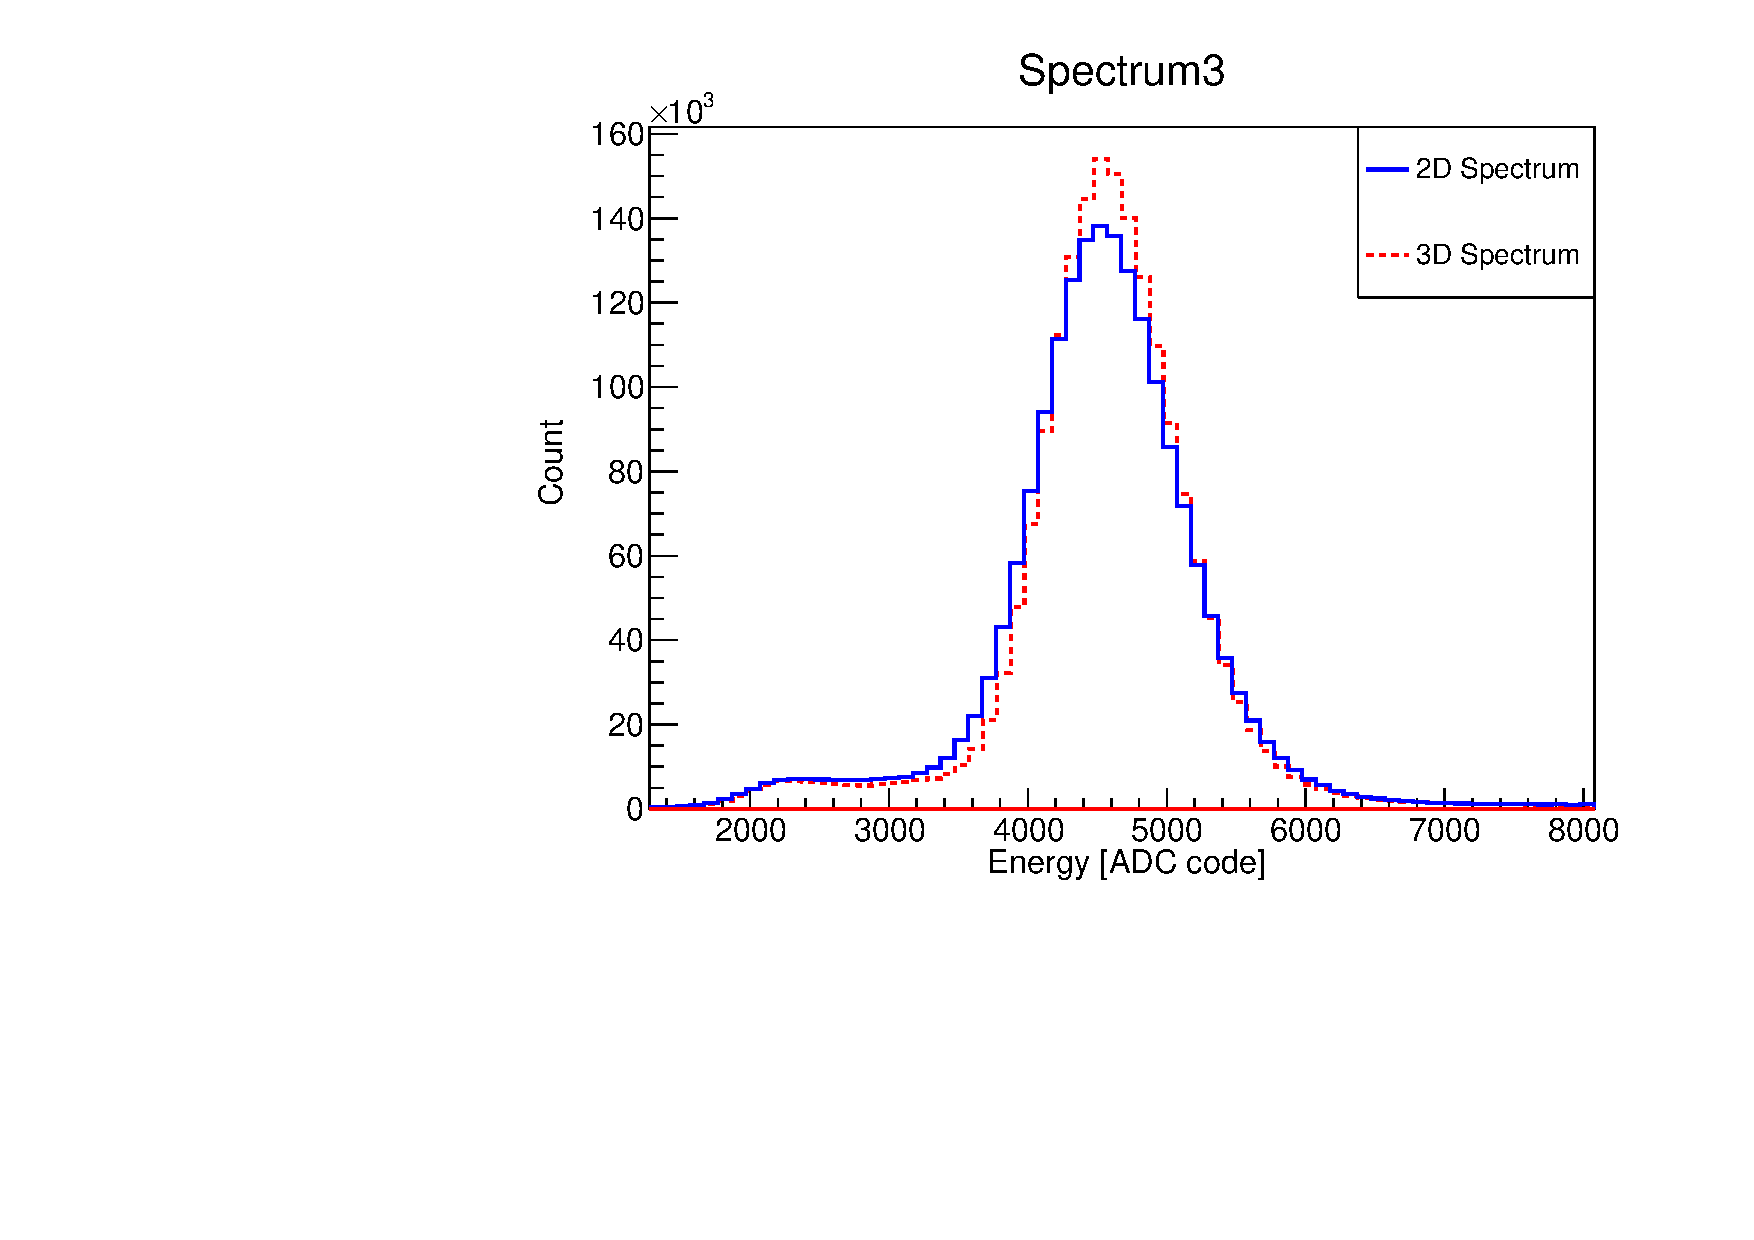
\includegraphics[width=0.65\textwidth]{20241103154350_signal_Fe55_CO2_540V_WV_16h_Spectrum.pdf}
    \caption{\ce{^{55}Fe} 源增益修正后能谱}
    \label{fig:Fe55EnergyFixed}
\end{figure}

将修正流程中的二维直方图绘制出来如图 \ref{fig:PixelEnergyDistribution} 所示,可作为 Micromegas 增益非均匀性的参考。

\begin{figure}[htbp]
    \centering
    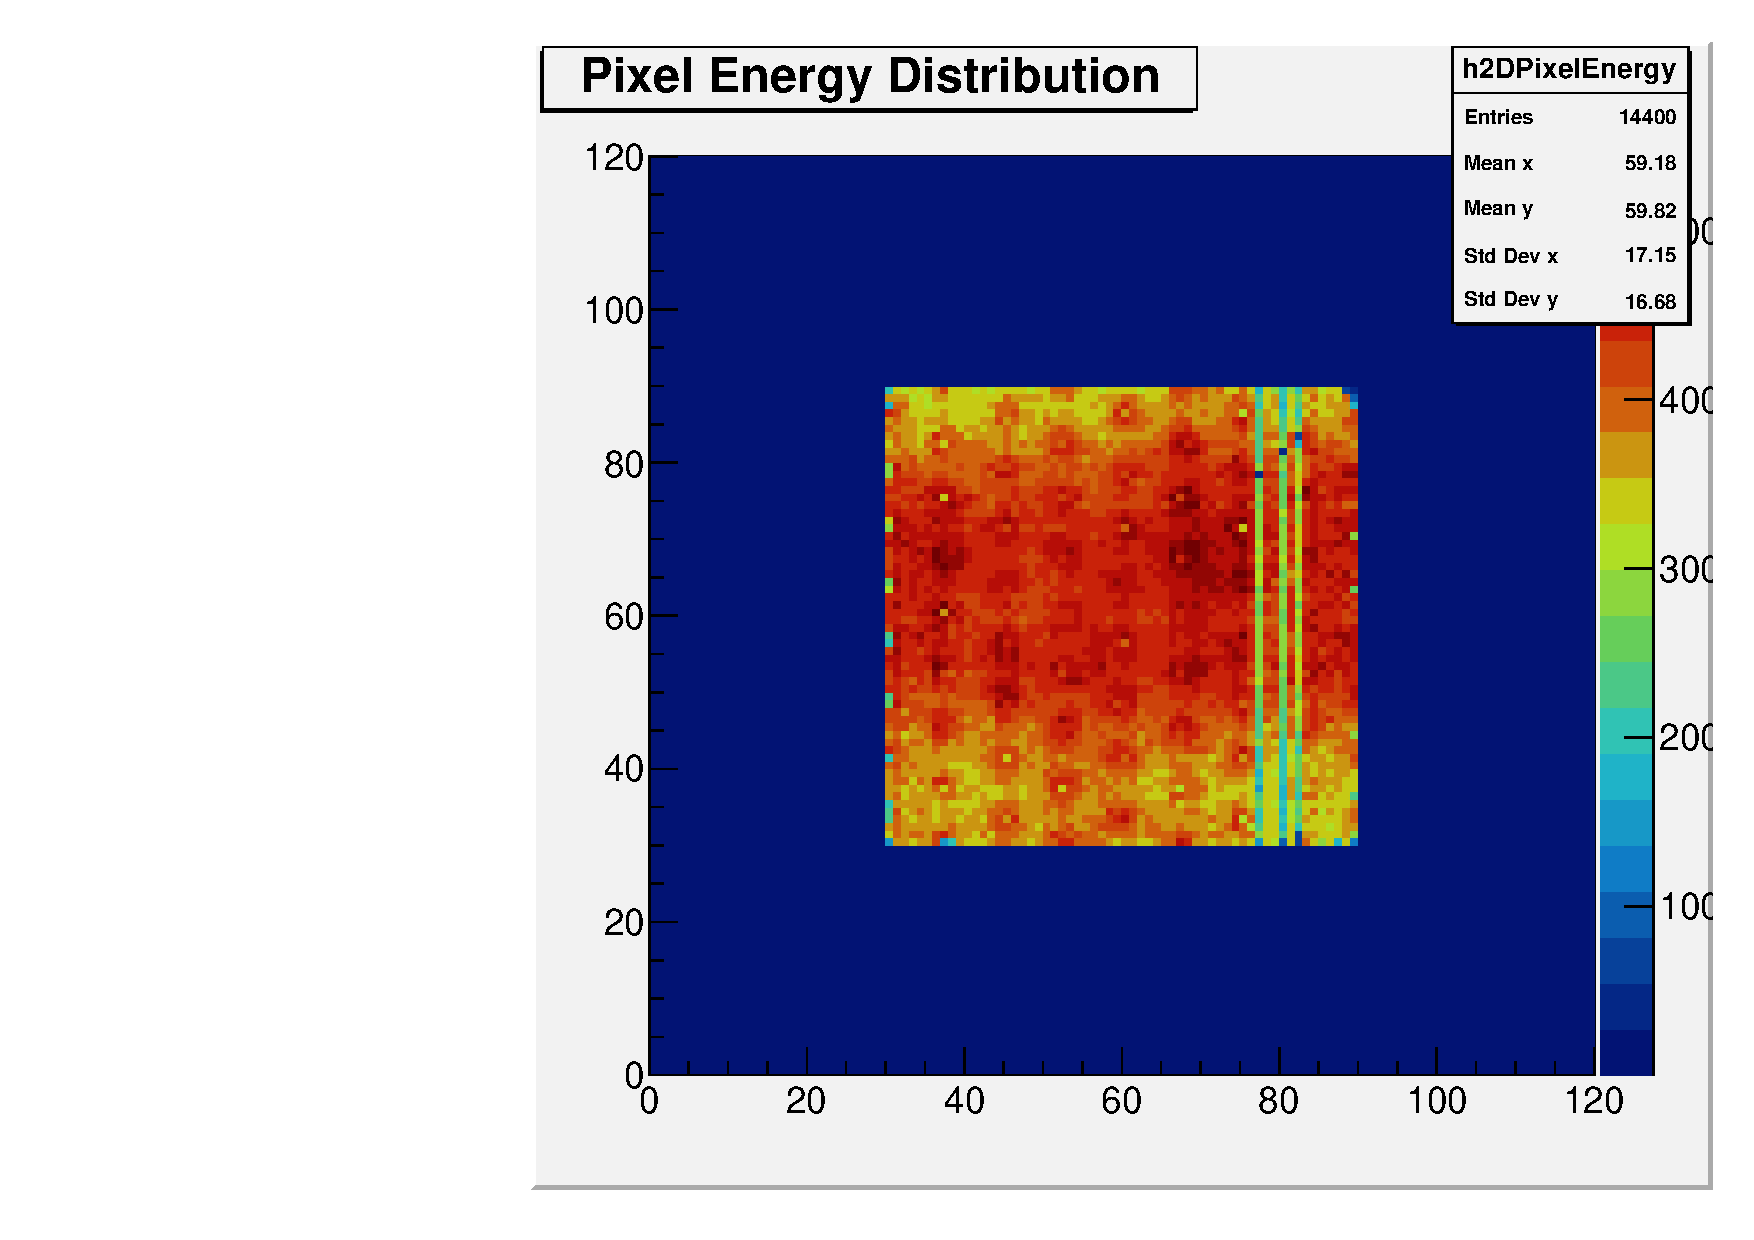
\includegraphics[width=0.65\textwidth]{20241103154350_signal_Fe55_CO2_540V_WV_16h_PixelEnergy.pdf}
    \caption{Micromegas 增益非均匀性参考}
    \label{fig:PixelEnergyDistribution}
\end{figure}

\subsection{进一步修正}
由于上述修正结果并不理想,考虑到 TPC 漂移区会对电子的扩散产生影响,因此通过调整漂移区的电场强度,增加电子收集效率,用于降低漂移区的影响,进一步修正 Micromegas 增益的非均匀性。修改漂移区电场强度后,\ce{^{55}Fe} 的能谱峰位变化不明显,说明 240 的雪崩区漂移区电场比较为合适。

考虑到测试 \ce{^{241}Am} 和 \ce{^{55}Fe} 所施加的雪崩区高压不同,增益不同,导致 Micromegas 增益非均匀性也会有所差异,使用 \ce{^{55}Fe} 的能谱进行修正可能导致过修正。因为探测器增益越大,非均匀性越大,\textbf{因此考虑对 \ce{^{55}Fe} 的能谱进行开 2.5 次根号处理},使其增益与 \ce{^{241}Am} 的增益接近,然后再进行修正。得到能量分辨率如图 \ref{fig:Am241Spectrum} 所示。

\begin{figure}[htbp]
    \centering
    \begin{subfigure}[t]{0.3\textwidth}
        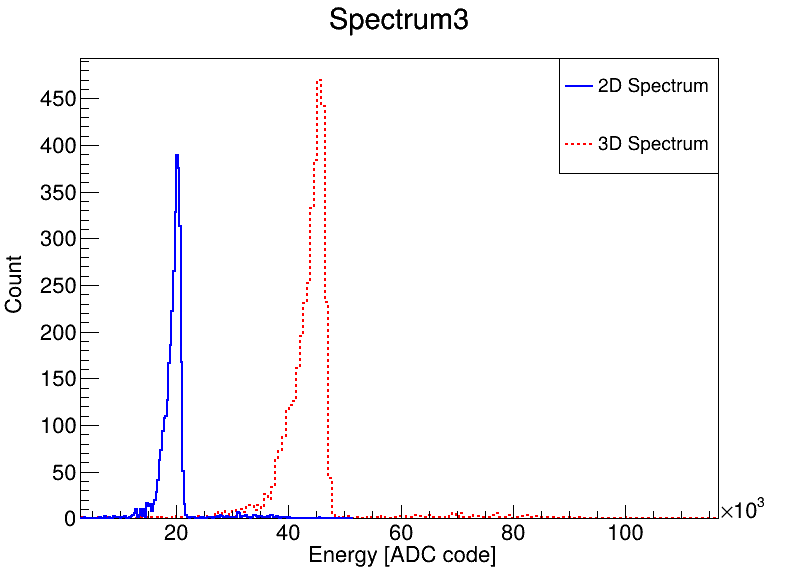
\includegraphics[width=\textwidth]{20240905093209_signal_Am241_inside_2min_Spectrum.png}
        \caption{\ce{^{241}Am} 修正前后能谱对比}
        \label{fig:Am241Comp}
    \end{subfigure}
    \hfill
    \begin{subfigure}[t]{0.3\textwidth}
        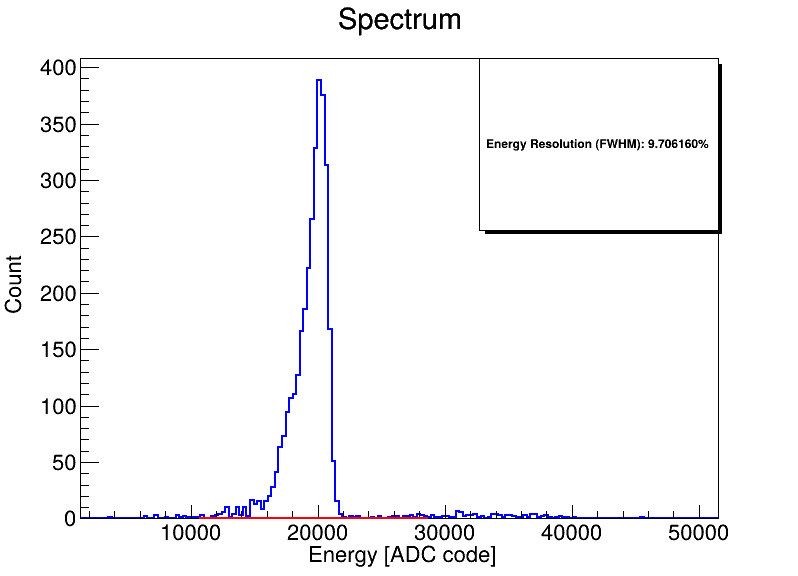
\includegraphics[width=\textwidth]{20240905093209_signal_Am241_inside_2min_2D.png}
        \caption{\ce{^{241}Am} 修正前能谱}
        \label{fig:Am241FixBefore}
    \end{subfigure}
    \hfill
    \begin{subfigure}[t]{0.3\textwidth}
        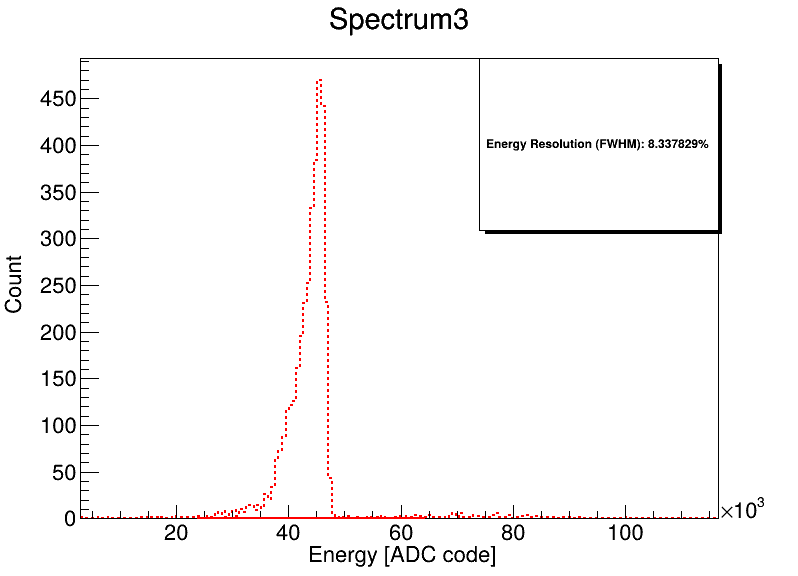
\includegraphics[width=\textwidth]{20240905093209_signal_Am241_inside_2min_3D.png}
        \caption{\ce{^{241}Am} 修正后能谱}
        \label{fig:Am241FixAfter}
    \end{subfigure}
    \caption{\ce{^{241}Am} 能谱修正结果}
    \label{fig:Am241Spectrum}
\end{figure}
